\documentclass[12pt]{standalone}
\usepackage{tikz}
\usetikzlibrary{patterns,matrix}

\begin{document}
%\begin{equation*}
%  B = \{P\in \mathbb{R}^2: d(O,P)\in [0,3) \cup (4,5)\},
%  \ C = \{P\in \mathbb{R}^2: d(O,P)\in [0,1) \cup (2,\infty)\}.
%\end{equation*}
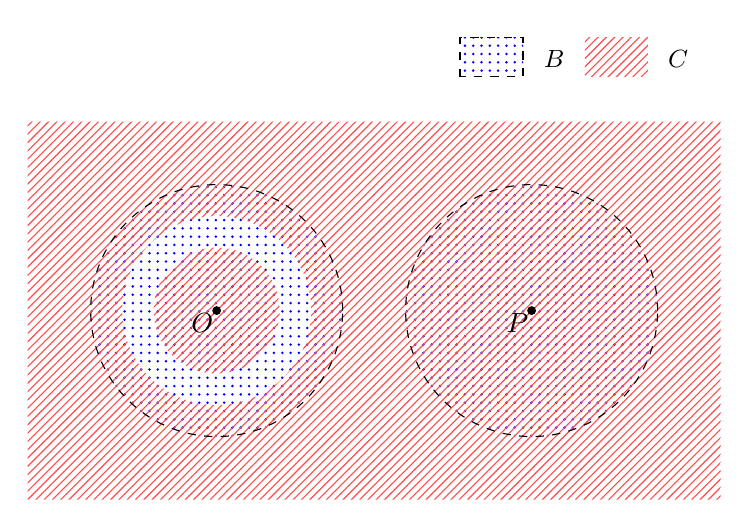
\begin{tikzpicture}[scale=0.8]
  %  \def\R{5}
  % B: blue fill
  \fill[pattern=dots,pattern color=blue] (0,0) circle (2);
  \fill[pattern=dots,pattern color=blue] (5,0) circle (2);
  % \fill[pattern=north west lines,pattern color=blue!70,even odd rule] (0,0) circle (5) (0,0) circle (4);
  % C: red hatching (unbounded, so clipped at radius \R)
  \fill[pattern=north east lines,pattern color=red!70] (0,0) circle (1);
  \fill[pattern=north east lines,pattern color=red!70,even odd rule]
    (-3,-3) rectangle (8,3) (0,0) circle (1.5);

  \foreach \r in {2} \draw[dashed] (0,0) circle (\r);
  \foreach \r in {2} \draw[dashed] (5,0) circle (\r);
  %\draw[dotted] (0,0) circle (\R);
  \fill (0,0) circle (2pt) node[below left,inner sep=1pt] {$O$};
  \fill (5,0) circle (2pt) node[below left,inner sep=1pt] {$P$};
  % radial scale
  % \draw[->] (0,0) -- (\R+0.7,0) node[right] {$d(O,P)$};
 % \foreach \r in {1,2,3,4,5} \draw (\r,2pt) -- (\r,-2pt) node[below,font=\footnotesize] {\r};
  % legend
  \matrix[anchor=north west,font=\small,row sep=2pt,column sep=4pt] at (3.7,4.5) {
    \fill[pattern=dots, pattern color=blue, draw=black,dashed] (0,0) rectangle (0.8,0.5); 
    & \node[anchor=south west]{$B$}; 
    &
    \fill[pattern=north east lines,pattern color=red!70] (0,0) rectangle (0.8,0.5); 
    & \node[anchor=south west]{$C$}; \\
  };
\end{tikzpicture}

\end{document}
